\appendix
\chapter{Type-safe differentiable programming}

\section{Grammar}

Below is an approximately complete BNF grammar for Kotlin$\nabla$:

\newcommand{\mor}{\ensuremath{\;\mid\;}}
\newcommand{\code}[1]{\ensuremath{\text{\inline{#1}}}}
\newcommand{\bnfrl}[1]{\ensuremath{\langle#1\rangle}}
\begin{eqnarray*}
    \bnfrl{type} & ::= & \code{Double} \mor \code{Float} \mor \code{Int} \mor \code{BigInteger} \mor \code{BigDouble} \\
    \bnfrl{nat} & ::= & \code{1} \mor \ldots \mor \code{99} \\
    \bnfrl{output} & ::= & \code{Fun<}\bnfrl{type}\code{Real>} \mor \code{VFun<}\bnfrl{type}\code{Real,}\bnfrl{nat}\code{>} \mor \code{MFun<}\bnfrl{type}\code{Real,}\bnfrl{nat}\code{,}\bnfrl{nat}\code{>} \\
    \bnfrl{int} & ::= & \code{0} \mor \bnfrl{nat}\bnfrl{int} \\
    \bnfrl{float} & ::= & \bnfrl{int}\code{.}\bnfrl{int} \\
    \bnfrl{num} & ::= & \bnfrl{type}\code{(}\bnfrl{int}\code{)} \mor \bnfrl{type}\code{(}\bnfrl{float}\code{)} \\
    \bnfrl{var} & ::= & \code{x} \mor \code{y} \mor \code{z} \mor \code{ONE} \mor \code{ZERO} \mor \code{E} \mor \code{Var()}} \\
\bnfrl{signOp} & ::= & \code{+} \mor \code{-} \\
\bnfrl{binOp} & ::= & \bnfrl{signOp} \mor \code{*} \mor \code{/} \mor \code{pow} \\
\bnfrl{trigOp} & ::= & \code{sin} \mor \code{cos} \mor \code{tan} \mor \code{asin} \mor \code{acos} \mor \code{atan} \mor \code{asinh} \mor \code{acosh} \mor \code{atanh} \\
\bnfrl{unaryOp} & ::= & \bnfrl{signOp} \mor \bnfrl{trigOp} \mor \code{sqrt} \mor \code{log} \mor \code{ln} \mor \code{exp} \\
\bnfrl{exp} & ::= & \bnfrl{var} \mor \bnfrl{num} \mor \bnfrl{unaryOp}\bnfrl{exp} \mor \bnfrl{var}\bnfrl{binOp}\bnfrl{exp} \mor \code{(} \bnfrl{exp} \code{)} \\
\bnfrl{expList} & ::= & \bnfrl{exp} \mor \bnfrl{exp} \code{,} \bnfrl{expList} \\
\bnfrl{linOp} & ::= & \bnfrl{signOp} \mor \code{*} \mor \code{ dot } \\
\bnfrl{vec} & ::= & \code{Vec(} \bnfrl{expList} \code{)} \mor \code{Vec} \bnfrl{nat} \code{(} \bnfrl{expList} \code{)} \\
\bnfrl{vecExp} & ::= & \bnfrl{vec} \mor \bnfrl{signOp}\bnfrl{vecExp} \mor \bnfrl{exp} \code{*} \bnfrl{vecExp} \mor \bnfrl{vec} \bnfrl{linOp} \bnfrl{vecExp} \\
&&\bnfrl{vecExp}\code{.norm(}\bnfrl{int}\code{)} \\
\bnfrl{mat} & ::= & \code{Mat} \bnfrl{nat} \code{x} \bnfrl{nat} \code{(} \bnfrl{expList} \code{)} \\
\bnfrl{matExp} & ::= & \bnfrl{mat} \mor \bnfrl{signOp}\bnfrl{matExp} \mor \bnfrl{exp}\bnfrl{linOp}\bnfrl{matExp} \mor \\
&&\bnfrl{vecExp}\bnfrl{linOp}\bnfrl{matExp} \mor \bnfrl{mat} \bnfrl{linOp} \bnfrl{matExp} \\
\bnfrl{anyExp} & ::= & \bnfrl{exp} \mor \bnfrl{vecExp} \mor \bnfrl{matExp} \mor \bnfrl{derivative} \mor \bnfrl{invocation} \\
\bnfrl{bindings} & ::= & \bnfrl{exp} \code{ to } \bnfrl{exp} \mor \bnfrl{exp} \code{ to } \bnfrl{exp} \code{,} \bnfrl{bindings} \\
\bnfrl{invocation} & ::= & \bnfrl{anyExp} \code{(} \bnfrl{bindings} \code{)} \\
\bnfrl{derivative} & ::= & \code{d(} \bnfrl{anyExp} \code{) / d(} \bnfrl{exp} \code{)} \mor \bnfrl{anyExp} \code{.d(} \bnfrl{exp} \code{)} \mor \bnfrl{anyExp} \code{.d(} \bnfrl{expList} \code{)} \\
\bnfrl{gradient} & ::= & \bnfrl{exp} \code{.grad()}
\end{eqnarray*}


\section{Linear regression}\label{sec:lin_reg}

\noindent Recall the matrix equation for linear regression, where $\mathbf{X}: \mathbb{R}^{m \times n}$ and $\bm\Theta: \mathbb{R}^{n \times 1}$:
%
\begin{equation}\label{eq:lin_reg}
\mathbf{\hat f}(\mathbf{X}; \bm\Theta) = \mathbf{X}\bm\Theta
\end{equation}
%
Imagine we are given the following dataset:
%
\begin{equation}
\mathbf{X} =
\begin{bmatrix}
\mathbf{x}_1 \\
\vdots \\
\mathbf{x}_m
\end{bmatrix} =
\begin{pmatrix}
1 & \ldots & x_{1n} \\
\vdots & \ddots & \vdots \\
1 & \ldots & x_{mn}
\end{pmatrix},
\mathbf{Y} =
\begin{bmatrix}
y_2 \\
\vdots \\
y_m
\end{bmatrix}
\end{equation}
%
Our goal in ordinary least squares (OLS) linear regression is to minimize the loss, or error between the data and the model's prediction:
%
\begin{equation}
\mathcal{L}(\mathbf{X}, \mathbf{Y}; \bm\Theta) = ||\mathbf{Y} - \mathbf{\hat f}(\mathbf{X}; \bm\Theta)||^2
\end{equation}
%
\begin{equation}
\bm\Theta^* = \underset{\bm\Theta}{\operatorname{argmin}}\mathcal{L}(\mathbf{X}, \mathbf{Y}; \bm\Theta)
\end{equation}

\subsection{Finite difference method}\label{sec:fdm}

First, we consider the scalar case, where $\mathbf{\hat f}(\mathbf{X}; \bm\Theta) = \hat f(x; \theta_2, \theta_1) = \theta_2 x + \theta_1$. Since $\mathbf{X}, \mathbf{Y}$ are considered to be fixed, we can rewrite $\mathcal{L}(\mathbf{X}, \mathbf{Y}; \bm\Theta)$ as simply:
%
\begin{equation}
\mathcal{L}(\bm\Theta) = \mathcal{L}(\theta_2, \theta_1) = \frac{1}{m}\sum_{i=1}^m(y_i - (\theta_2 x_i + \theta_1))^2
\end{equation}
%
To find the minimizer of $\mathcal{L}(\bm\Theta)$, we need $\nabla_{\bm\Theta}\mathcal{L} = \lbrack \frac{\partial\mathcal{L}}{\partial \theta_2}, \frac{\partial\mathcal{L}}{\partial \theta_1}\rbrack$. There are various ways to compute this. First, let's see FDM with centered differences:
%
\begin{align}
\frac{\partial\mathcal{L}}{\partial \theta_1} & = \underset{h \rightarrow 0}{\operatorname{lim}} \frac{\sum_{i=1}^m\left(y_i - \left(\theta_2 x_i + \theta_1 + h\right)\right)^2 - \sum_{i=1}^m\left(y_i - \left(\theta_2 x_i + \theta_1 - h\right)\right)^2}{2hm} \\ & = \underset{h \rightarrow 0}{\operatorname{lim}} \frac{1}{2hm}\sum_{i=1}^m\left(y_i - \left(\theta_2 x_i + \theta_1 + h\right)\right)^2 - \left(y_i - \left(\theta_2 x_i + \theta_1 - h\right)\right)^2 \\
\frac{\partial\mathcal{L}}{\partial \theta_2} & = \underset{h \rightarrow 0}{\operatorname{lim}} \frac{\sum_{i=1}^m\left(y_i - \left((\theta_2 + h) x_i + \theta_1\right)\right)^2 - \sum_{i=1}^m\left(y_i - \left(\left(\theta_2 - h\right) x_i + \theta_1\right)\right)^2}{2hm} \\ & = \underset{h \rightarrow 0}{\operatorname{lim}} \frac{1}{2hm}\sum_{i=1}^m\left(y_i - \left(\left(\theta_2 + h\right) x_i + \theta_1\right)\right)^2 - \left(y_i - \left(\left(\theta_2 - h\right) x_i + \theta_1\right)\right)^2
\end{align}
%
Using computer algebra, the above equations can be simplified considerably:
%
\begin{align}
\frac{\partial\mathcal{L}}{\partial \theta_1} & = \underset{h \rightarrow 0}{\operatorname{lim}} \frac{1}{2hm}\sum_{i=1}^m\left(4h ( \theta_1 +  \theta_2 x_i - y_i)\right) \label{eq:dL_dtheta0} \\
& = \boxed{\frac{2}{m}\sum_{i=1}^m\left(\theta_1 + \theta_2 x_i - y_i\right)} \\
\frac{\partial\mathcal{L}}{\partial \theta_2} & = \underset{h \rightarrow 0}{\operatorname{lim}} \frac{1}{2hm}\sum_{i=1}^m\left(4hx_i (\theta_2 x_i + \theta_1 - y_i)\right) \label{eq:dL_dtheta1} \\
& = \boxed{\frac{2}{m}\sum_{i=1}^m(x_i)(\theta_2 x_i + \theta_1 - y_i)}
\end{align}
%
\begin{enumerate}
\item[] \autoref{eq:dL_dtheta0}: \url{https://www.wolframalpha.com/input/?i=(y_i-((%CE%B8_2%2Bh)x_i%2B%CE%B8_1))%5E2-(y_i-((%CE%B8_2-h)x_i%2B%CE%B8_1))%5E2}
\item[] \autoref{eq:dL_dtheta1}: \url{https://www.wolframalpha.com/input/?i=(y_i-(%CE%B8_2*x_i%2B%CE%B8_1%2Bh))%5E2%E2%88%92(y_i-(%CE%B8_2*x_i%2B%CE%B8_1-h))%5E2}
\end{enumerate}

\subsection{Partial differentiation}

\noindent Alternatively, we can calculate the partials analytically, by applying the chain rule:
%
\begin{align}
\frac{\partial\mathcal{L}}{\partial \theta_1} & = \frac{\partial}{\partial \theta_1}\frac{1}{m}\sum_{i=1}^m(y_i - (\theta_2 x_i + \theta_1))^2 \\ & = \frac{1}{m}\sum_{i=1}^m 2 (y_i - (\theta_2 x_i + \theta_1))\frac{\partial}{\partial \theta_1}(y_i - (\theta_2 x_i + \theta_1)) \\ & = \frac{2}{m}\sum_{i=1}^m(y_i - (\theta_2 x_i + \theta_1))(-1) \\ & = \boxed{\frac{2}{m}\sum_{i=1}^m(\theta_2 x_i + \theta_1 - y_i)}
\end{align}
%
\begin{align}
\frac{\partial\mathcal{L}}{\partial \theta_2} & = \frac{\partial}{\partial \theta_2}\frac{1}{m}\sum_{i=1}^m(y_i - (\theta_2 x_i + \theta_1))^2 \\ & = \frac{1}{m}\sum_{i=1}^m 2(y_i - (\theta_2 x_i + \theta_1)) \frac{\partial}{\partial \theta_2}(y_i - (\theta_2 x_i + \theta_1)) \\ & = \frac{2}{m}\sum_{i=1}^m(y_i - (\theta_2 x_i + \theta_1))(-x_i) \\ & = \boxed{\frac{2}{m}\sum_{i=1}^m(x_i)(\theta_2 x_i + \theta_1 - y_i)}
\end{align}
%
Notice how analytical differentiation gives us the same answer as the \hyperref[sec:fdm]{finite difference method} (this is not by accident), with much less algebra. We can rewrite these two solutions in gradient form, i.e. as a column vector of partial derivatives:
%
\begin{equation}
\nabla_{\bm\Theta}\mathcal{L} =
\begin{bmatrix}
\frac{\partial\mathcal{L}}{\partial \theta_1} \\
\frac{\partial\mathcal{L}}{\partial \theta_2}
\end{bmatrix} = \frac{2}{m}
\begin{bmatrix}
\sum_{i=1}^m(\theta_2 x_i + \theta_1 - y_i) \\ \sum_{i=1}^m(x_i)(\theta_2 x_i + \theta_1 - y_i)
\end{bmatrix}
\end{equation}

\subsection{Matrix solution}\label{sec:linreg_matrix_sol}

Having reviewed the scalar procedure for linear regression, let us now return to the general form of $\mathcal L(\bm\Theta)$. Matrix notation allows us to simplify the loss considerably:
%
\begin{align}
\mathcal L(\bm\Theta) & = \frac{1}{m} (\mathbf Y - \mathbf X \bm\Theta)^\intercal(\mathbf Y - \mathbf X \bm\Theta) \\ &= \frac{1}{m} (\mathbf Y^\intercal \mathbf Y - \mathbf Y^\intercal \mathbf X \bm\Theta - \bm\Theta^\intercal \mathbf X^\intercal \mathbf Y + \bm\Theta^\intercal \mathbf X^\intercal \mathbf X \bm\Theta) \\ &= \frac{1}{m} (\mathbf Y^\intercal \mathbf Y - 2 \bm\Theta^\intercal \mathbf X^\intercal \mathbf Y + \bm\Theta^\intercal \mathbf X^\intercal \mathbf X \bm\Theta)
\end{align}
%
Matrix notation allows us to derive the gradient and requires far less algebra:
%
\begin{align}
\nabla_{\bm\Theta}\mathcal L(\bm\Theta) & = \frac{1}{m} (\nabla_{\bm\Theta}\mathbf Y^\intercal \mathbf Y - 2 \nabla_{\bm\Theta} \bm\Theta^\intercal \mathbf X^\intercal \mathbf Y + \nabla_{\bm\Theta}\bm\Theta^\intercal \mathbf X^\intercal \mathbf X \bm\Theta) \\ & = \frac{1}{m} ( 0 - 2\mathbf{X}^\intercal \mathbf Y + 2 \mathbf{X}^\intercal \mathbf X \bm\Theta ) \\ & = \boxed{\frac{2}{m} (\mathbf{X}^\intercal \mathbf X \bm\Theta - \mathbf{X}^\intercal \mathbf Y)}
\end{align}
%
For completeness, and to convince ourselves the matrix solution is indeed the same:
%
\begin{align}
& = \frac{2}{m}\left(
\underbrace{\begin{bmatrix}
1 & \ldots & 1 \\
x_1 & \ldots & x_m \\
\end{bmatrix}}_{\mathbf{X}^\intercal}
\underbrace{\begin{bmatrix}
1 & x_1 \\
\vdots & \vdots \\
1 & x_m
\end{bmatrix}}_{\mathbf{X}}
\underbrace{\begin{bmatrix}
\theta_1 \\
\theta_2
\end{bmatrix}}_{\bm\Theta} -
\underbrace{\begin{bmatrix}
1 & \ldots & 1 \\
x_1 & \ldots & x_m \\
\end{bmatrix}}_{\mathbf{X}^\intercal}
\underbrace{\begin{bmatrix}
y_1 \\
\vdots \\
y_m
\end{bmatrix}}_{\mathbf{Y}}\right) \\
& = \frac{2}{m}\left(
\underbrace{\begin{bmatrix}
m & \sum_{i=1}^{m}x_i \\
\sum_{i=1}^{m}x_i & \sum_{i=1}^{m}x_i^2 \\
\end{bmatrix}}_{\mathbf{X}^\intercal\mathbf{X}}
\underbrace{\begin{bmatrix}
\theta_1 \\
\theta_2
\end{bmatrix}}_{\bm\Theta} -
\underbrace{\begin{bmatrix}
\sum_{i=1}^{m}y_i \\
\sum_{i=1}^{m}x_iy_i
\end{bmatrix}}_{\mathbf{X}^\intercal\mathbf{Y}}\right) \\
& = \frac{2}{m}\left(
\underbrace{\begin{bmatrix}
m \theta_1 + \sum_{i=1}^{m}\theta_2x_i \\
\sum_{i=1}^{m}\theta_1x_i + \sum_{i=1}^{m}\theta_2x_i^2
\end{bmatrix}}_{\mathbf{X}^\intercal\mathbf{X}\bm\Theta} -
\underbrace{\begin{bmatrix}
\sum_{i=1}^{m}y_i \\
\sum_{i=1}^{m}x_iy_i
\end{bmatrix}}_{\mathbf{X}^\intercal\mathbf{Y}}\right) \\
& = \boxed{\frac{2}{m}
\underbrace{\begin{bmatrix}
\sum_{i=1}^{m}\theta_2x_i + \theta_1 - y_i \\
\sum_{i=1}^{m}(x_i)(\theta_2x_i + \theta_1 - y_i)
\end{bmatrix}}_{\mathbf{X}^\intercal\mathbf{X}\bm\Theta - \mathbf{X}^\intercal\mathbf{Y}} =
\begin{bmatrix}
\frac{\partial\mathcal{L}}{\partial \theta_1} \\
\frac{\partial\mathcal{L}}{\partial \theta_2}
\end{bmatrix} = \nabla_{\bm\Theta}\mathcal{L}(\bm\Theta)}
\end{align}
%
Notice how we recover the same solution obtained from partial differentiation and finite difference approximation, albeit in a more compact form. For a good introduction to matrix calculus, the textbook by \citet{magnus2019matrix} is an excellent guide, of which \citet{petersen2012matrix} offer a review of important identities.

OLS linear regression is a convex optimization problem. If $\mathbf X^\intercal \mathbf X$ is invertible, i.e. full-rank, this implies a unique solution $\bm\Theta^*$, which we can solve for directly by setting $\nabla_{\bm\Theta}\mathcal{L} = \mathbf{0}$:
%
\begin{align}
\mathbf{0} & = \mathbf X^\intercal \mathbf X \bm \Theta - \mathbf X ^ \intercal \mathbf Y \\ \bm\Theta &= (\mathbf X^\intercal \mathbf X)^{-1}\mathbf X^\intercal\mathbf Y
\end{align}
%
Solving this requires computing $(\mathbf{X}^\intercal\mathbf{X})^{-1}$ which is at least $\mathcal{O}(n^{2.373})$\citep{williams2014multiplying} to the best of our knowledge, i.e. quadratic with respect to the number of input dimensions. Another way to find $\bm \Theta^*$ is by initializing $\bm\Theta \leftarrow \mathbf{0}$ and repeating the following procedure until convergence:
%
\begin{equation}
\bm\Theta' \leftarrow \bm\Theta - \alpha \nabla_{\bm\Theta}\mathcal L(\bm\Theta)
\end{equation}
%
Typically, $\alpha \in [0.001, 0.1]$. Although hyperparameter tuning is required to find a suitable $\alpha$ (various improvements like Nesterov momentum~\citep{nesterov2013gradient} and quasi-Newton methods also help to accelerate convergence), this procedure is guaranteed to be computationally more efficient than matrix inversion for sufficiently large $m$ and $n$. In practice, the normal equation is seldom used unless $m$ is very small.

\section{Polynomial regression}\label{sec:poly_reg}

Polynomial regression is a straightforward application of linear regression, where the weights are the coefficients for each term in a polynomial. Consider the univariate case:

\begin{equation}
y_i \,=\, \beta_0 + \beta_1 x_i + \beta_2 x_i^2 + \cdots + \beta_m x_i^m = \sum_{j=0}^{m} \beta_j x_i^{j}
\end{equation}
%
We can rewrite this function in matrix form as follows:
%
\begin{equation}
\begin{bmatrix} y_1\\ y_2\\ y_3 \\ \vdots \\ y_n \end{bmatrix}= \begin{bmatrix} 1 & x_1 & x_1^2 & \dots & x_1^m \\ 1 & x_2 & x_2^2 & \dots & x_2^m \\ 1 & x_3 & x_3^2 & \dots & x_3^m \\ \vdots & \vdots & \vdots & \ddots & \vdots \\ 1 & x_n & x_n^2 & \dots & x_n^m \end{bmatrix} \begin{bmatrix} \beta_0\\ \beta_1\\ \beta_2\\ \vdots \\ \beta_m \end{bmatrix}
\end{equation}
%
\begin{equation}
\mathbf{\hat f}_{PR}(\mathbf{X}; \bm\beta) = \mathbf{X}\bm\beta
\end{equation}
%
The resemblance to ~\autoref{eq:lin_reg} should be clear. To find $\bm\beta$ minimizing $\mathcal L(\mathbf{X}, \mathbf{Y};\bm\beta)$, we can use the same method described in ~\autoref{sec:linreg_matrix_sol}.

\chapter{Tools for reproducible robotics}

\section{Useful Docker resources}

The following resources have proven particularly helpful during the development of Duckietown's container infrastructure.

\subsection{\href{https://www.balena.io/}{Balena}}\label{subsec:balena}

Balena is a very good source of base images for ARM devices. The best part of using Balena images, is that they can be rebuilt on x86 devices, such as a laptop or cloud server. Baked into every Balena image is a shim for the shell that will allow users to run ARM binaries on x86 from inside a container. To use this feature, the following \inline{Dockerfile} template is provided:
%
\begin{dockerlisting}
FROM balena/BASE_IMAGE # e.g. raspberrypi3-python
RUN [ "cross-build-start" ]
# ARM-specific code goes here...
RUN [ "cross-build-end" ]
CMD <DEFAULT_START_COMMAND>
\end{dockerlisting}
%
Balena uses \href{https://www.qemu.org/}{QEMU}~\citep{bellard2005qemu} to cross-build images.\hspace{-.08em}\footnote{\url{https://www.balena.io/blog/building-arm-containers-on-any-x86-machine-even-dockerhub/}} When running an ARM image, simply use the \inline{qemu-arm-static} binary as a custom entrypoint:
%
\begin{pclisting}
~$ docker run (*@\hl{--entrypoint=qemu-arm-static}@*) -it your/arm-image bash
\end{pclisting}

\subsection{\href{https://hub.docker.com/_/ros}{ROS Docker Images}}

ROS.org builds nightly ARM and x86 images for robotics development. For each distribution, there are packages like \inline{core}, \inline{base}, \inline{perception} (including \href{https://opencv.org/}{OpenCV}), \inline{robot} and others.\vspace{10pt}
%
\begin{centering}
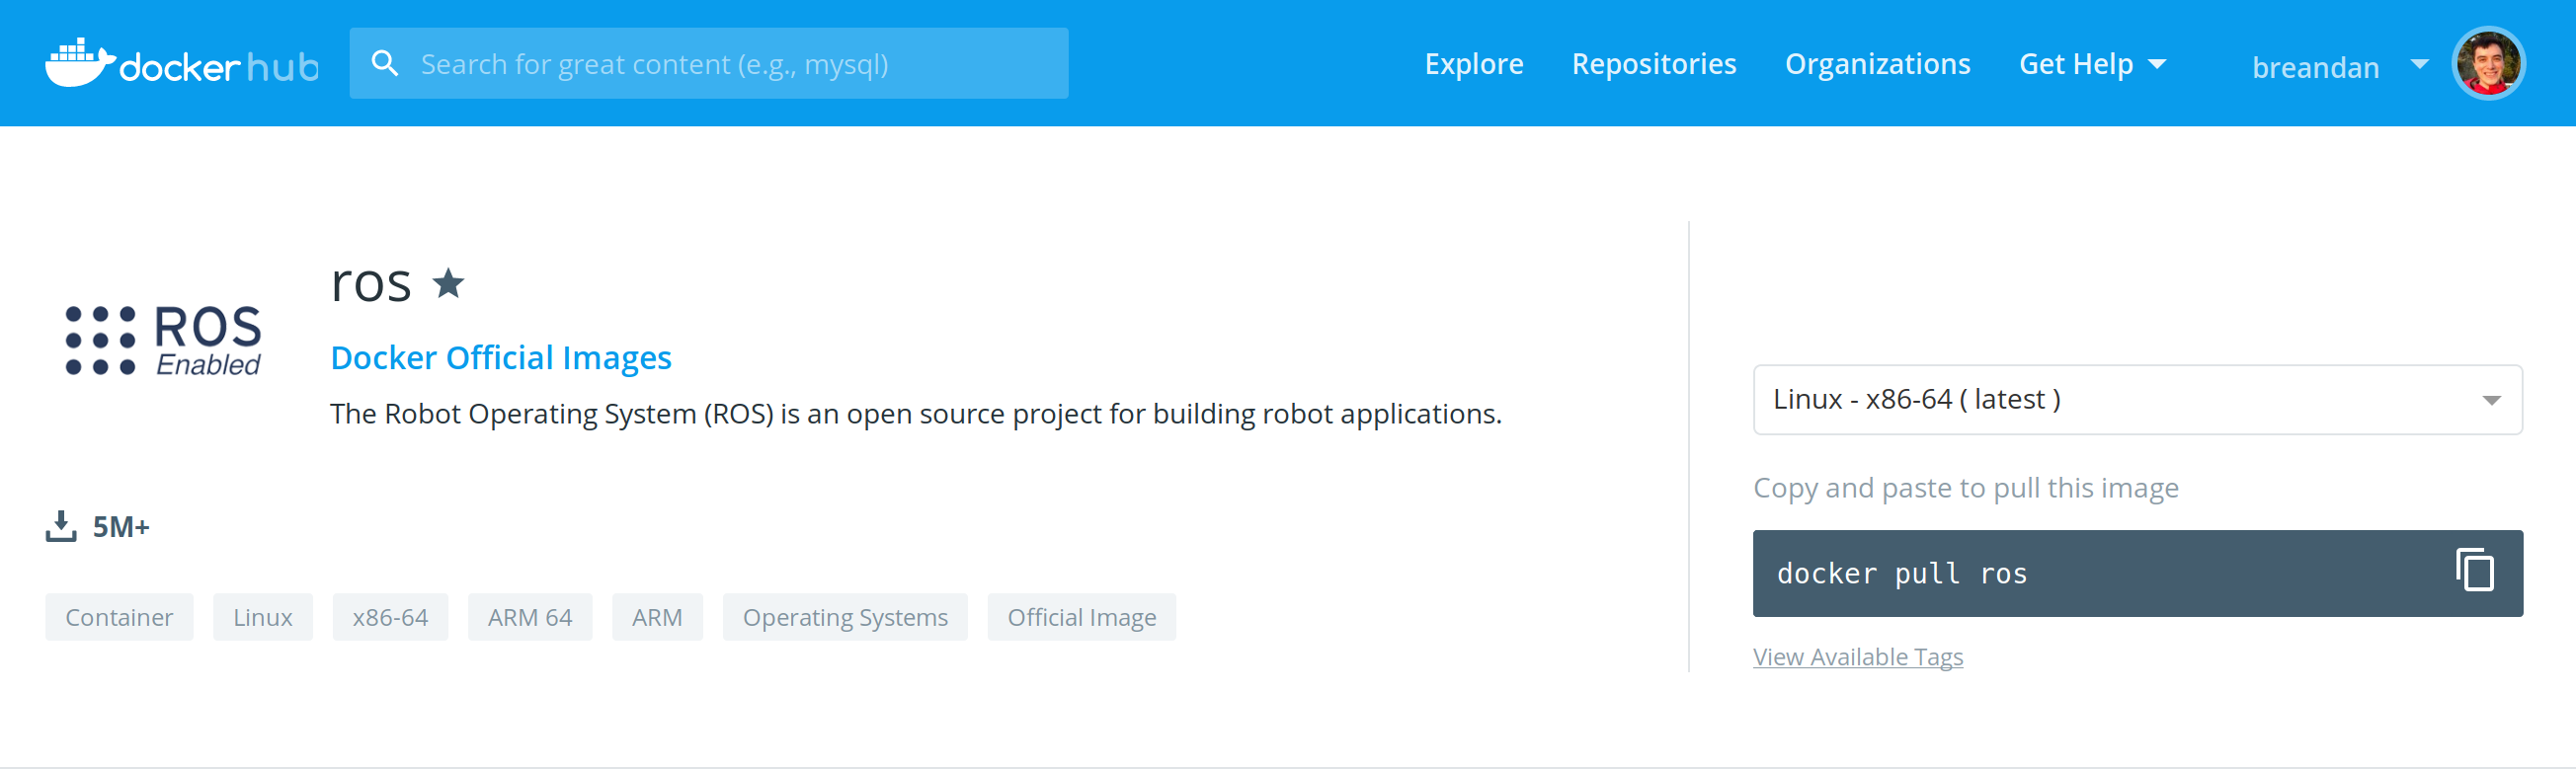
\includegraphics[width=\textwidth]{../figures/ros_docker_images.png}
\end{centering}

\subsection{\href{https://blog.hypriot.com/}{Hypriot}}\label{subsec:hypriot}

Hypriot, a base OS for RPi and other ARM devices, includes support for Docker straight out of the box. Hypriot is a lightweight Raspbian-based Linux distribution which \href{https://github.com/hypriot/image-builder-rpi}{builds} from the latest Raspberry Pi kernels and Raspbian releases.

\subsection{\href{https://www.piwheels.org/}{PiWheels}}

Not all Python packages (especially if they wrap a native library) can be run on all platforms. One might be tempted to build some package from its sources (and in rare cases, they might need to do so). But there is a good chance the package has already been compiled for Raspberry Pi on PiWheels. By using the following command (either in a \inline{Dockerfile} or via the CLI), various Python packages may be installed, e.g. \inline{opencv-python}:
%
\begin{rpilisting}
~$ pip install opencv-python --index-url https://www.piwheels.org/simple
\end{rpilisting}

\subsection{\href{https://hub.docker.com/}{Docker Hub}}\label{subsec:docker_hub}

Docker Hub is the central repository for Docker Images. Unless a separate registry has been configured, whenever users pull a Docker image tag, it will first query the Docker Hub for a matching image. The Docker Hub can be used to upload Docker images, and configure automated builds from GitHub (with a two hour build timeout). Docker Hub does not support layer caching of any kind, so the build will always take a fixed amount of time.\vspace{10pt}
%
\begin{centering}
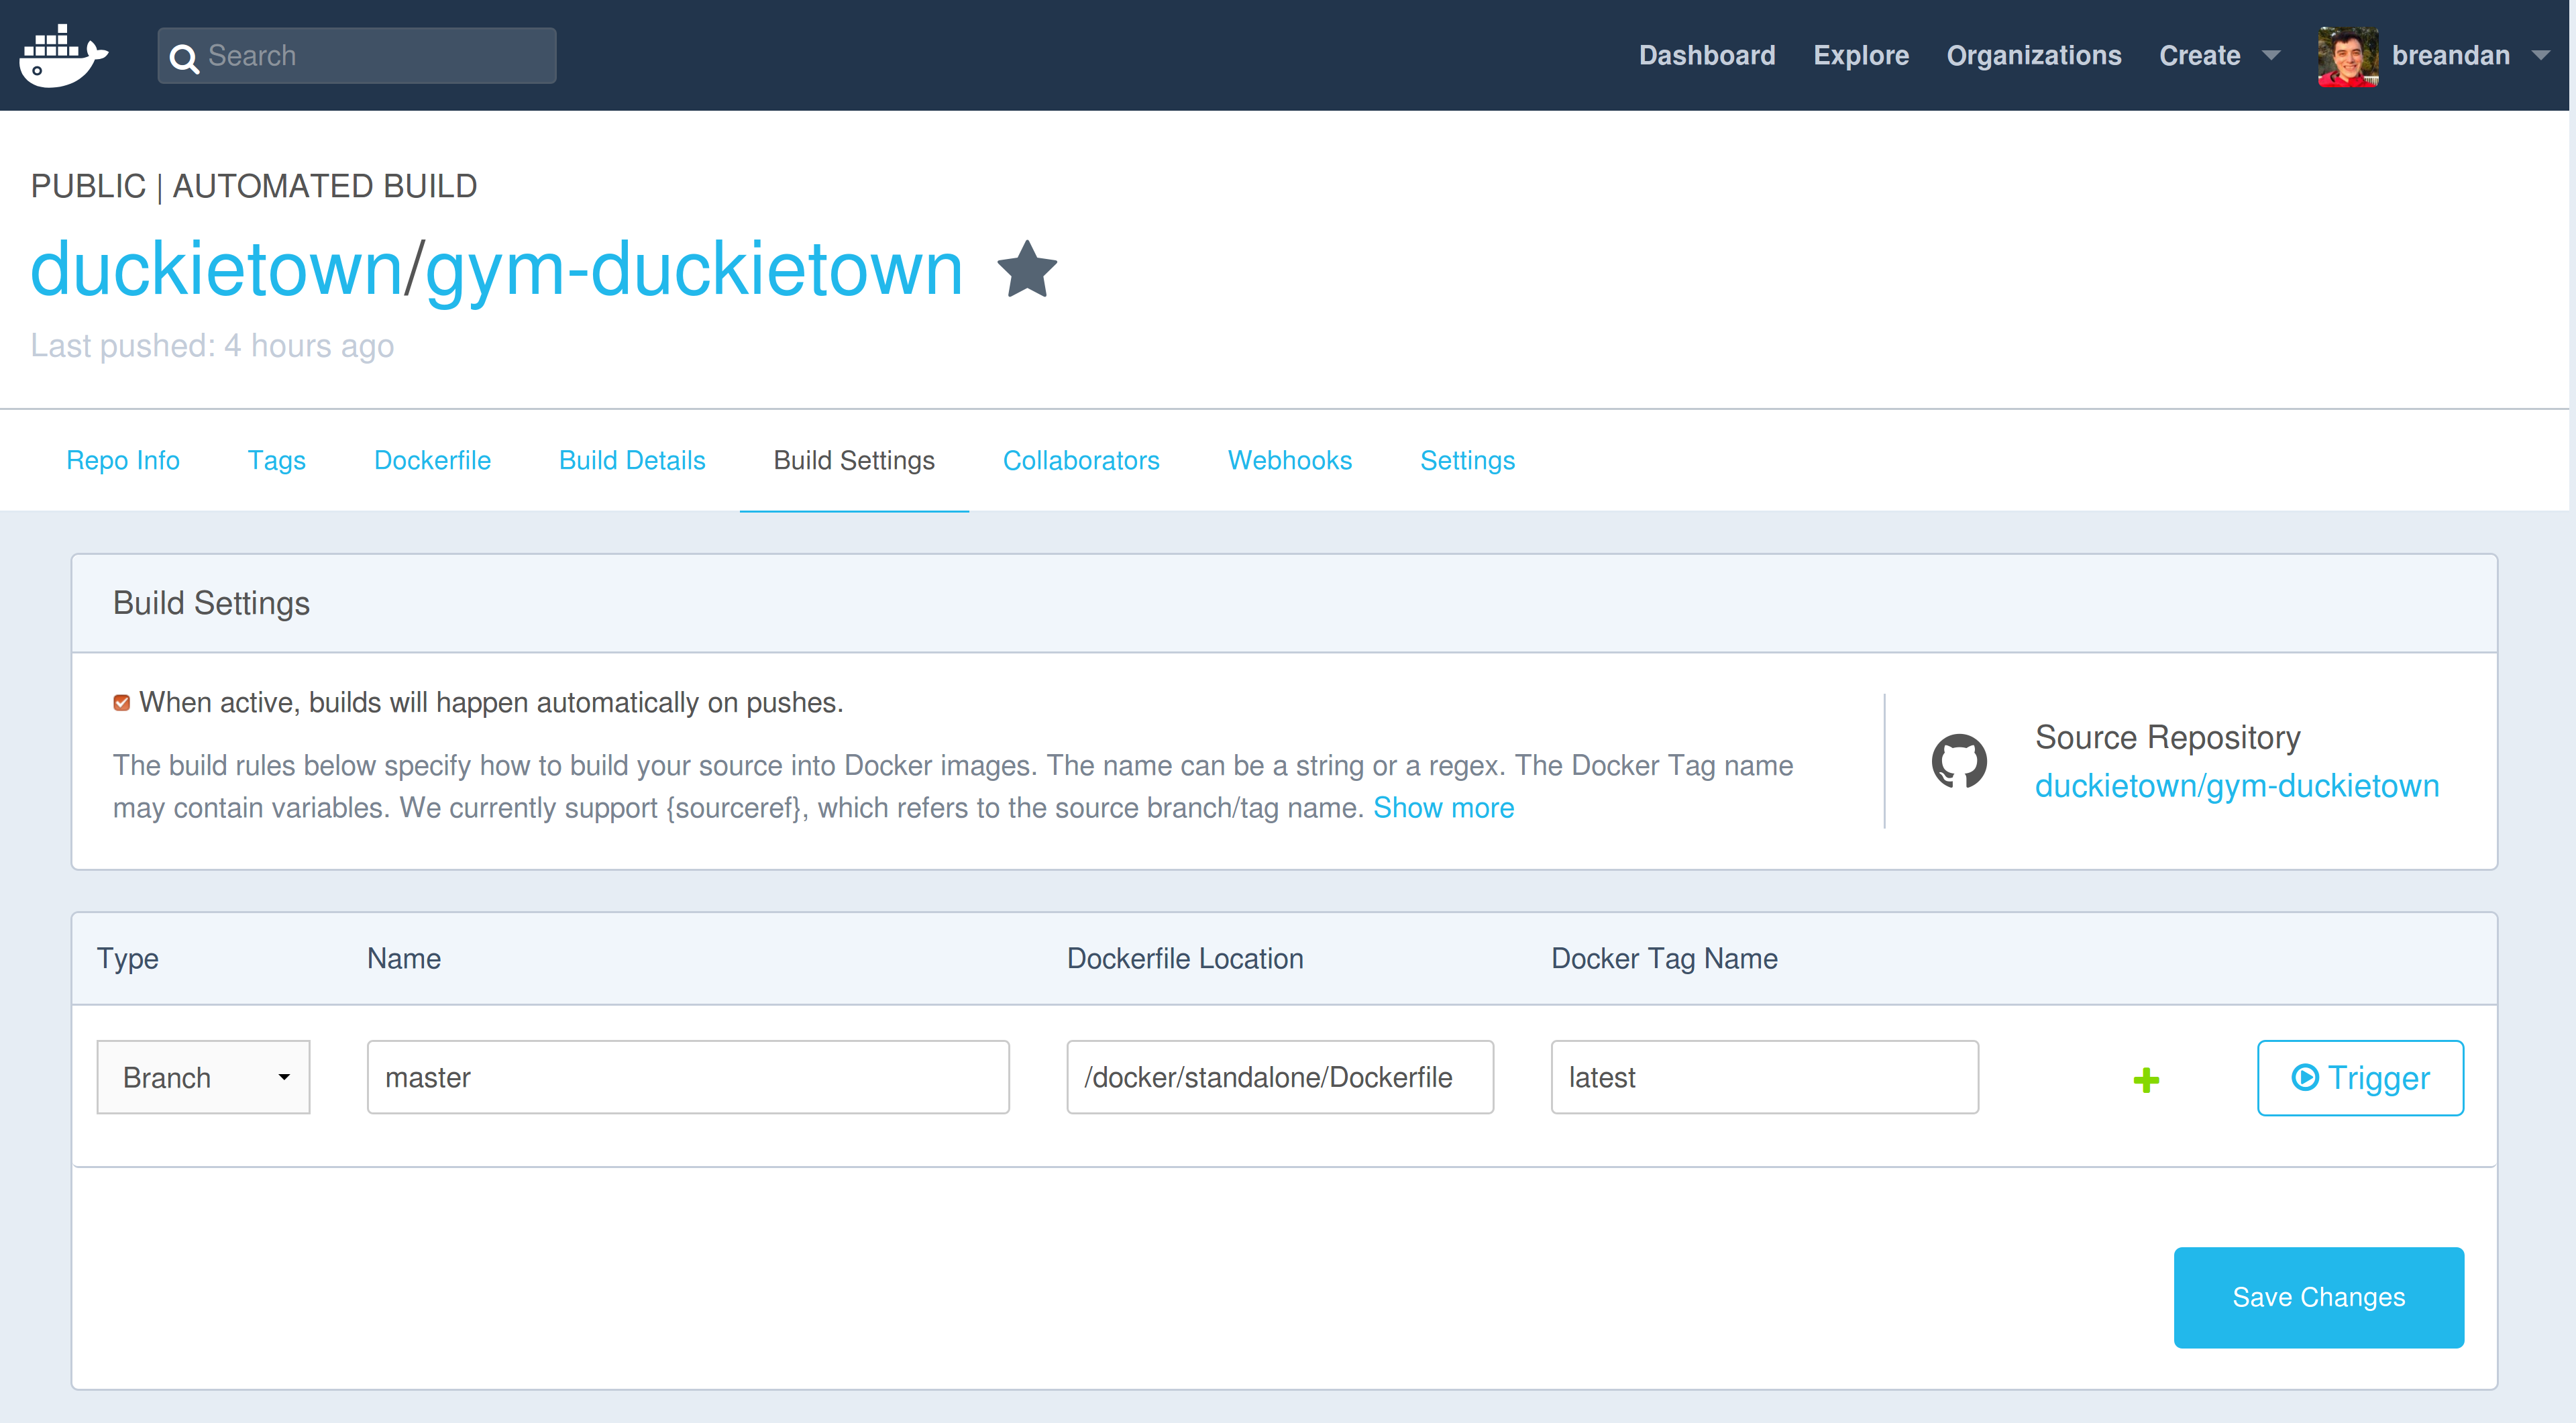
\includegraphics[width=\textwidth]{../figures/docker_hub_autobuild.png}
\end{centering}
%
Docker Hub auto-builds support linking a \inline{Dockerfile} in a GitHub repository, and whenever that \inline{Dockerfile} changes, the Docker image will be updated.

The Docker Hub also has features for configuring repository links and build triggers. These will automatically rebuild downstream Docker images whenever some event occurs.\vspace{10pt}
%
\begin{centering}
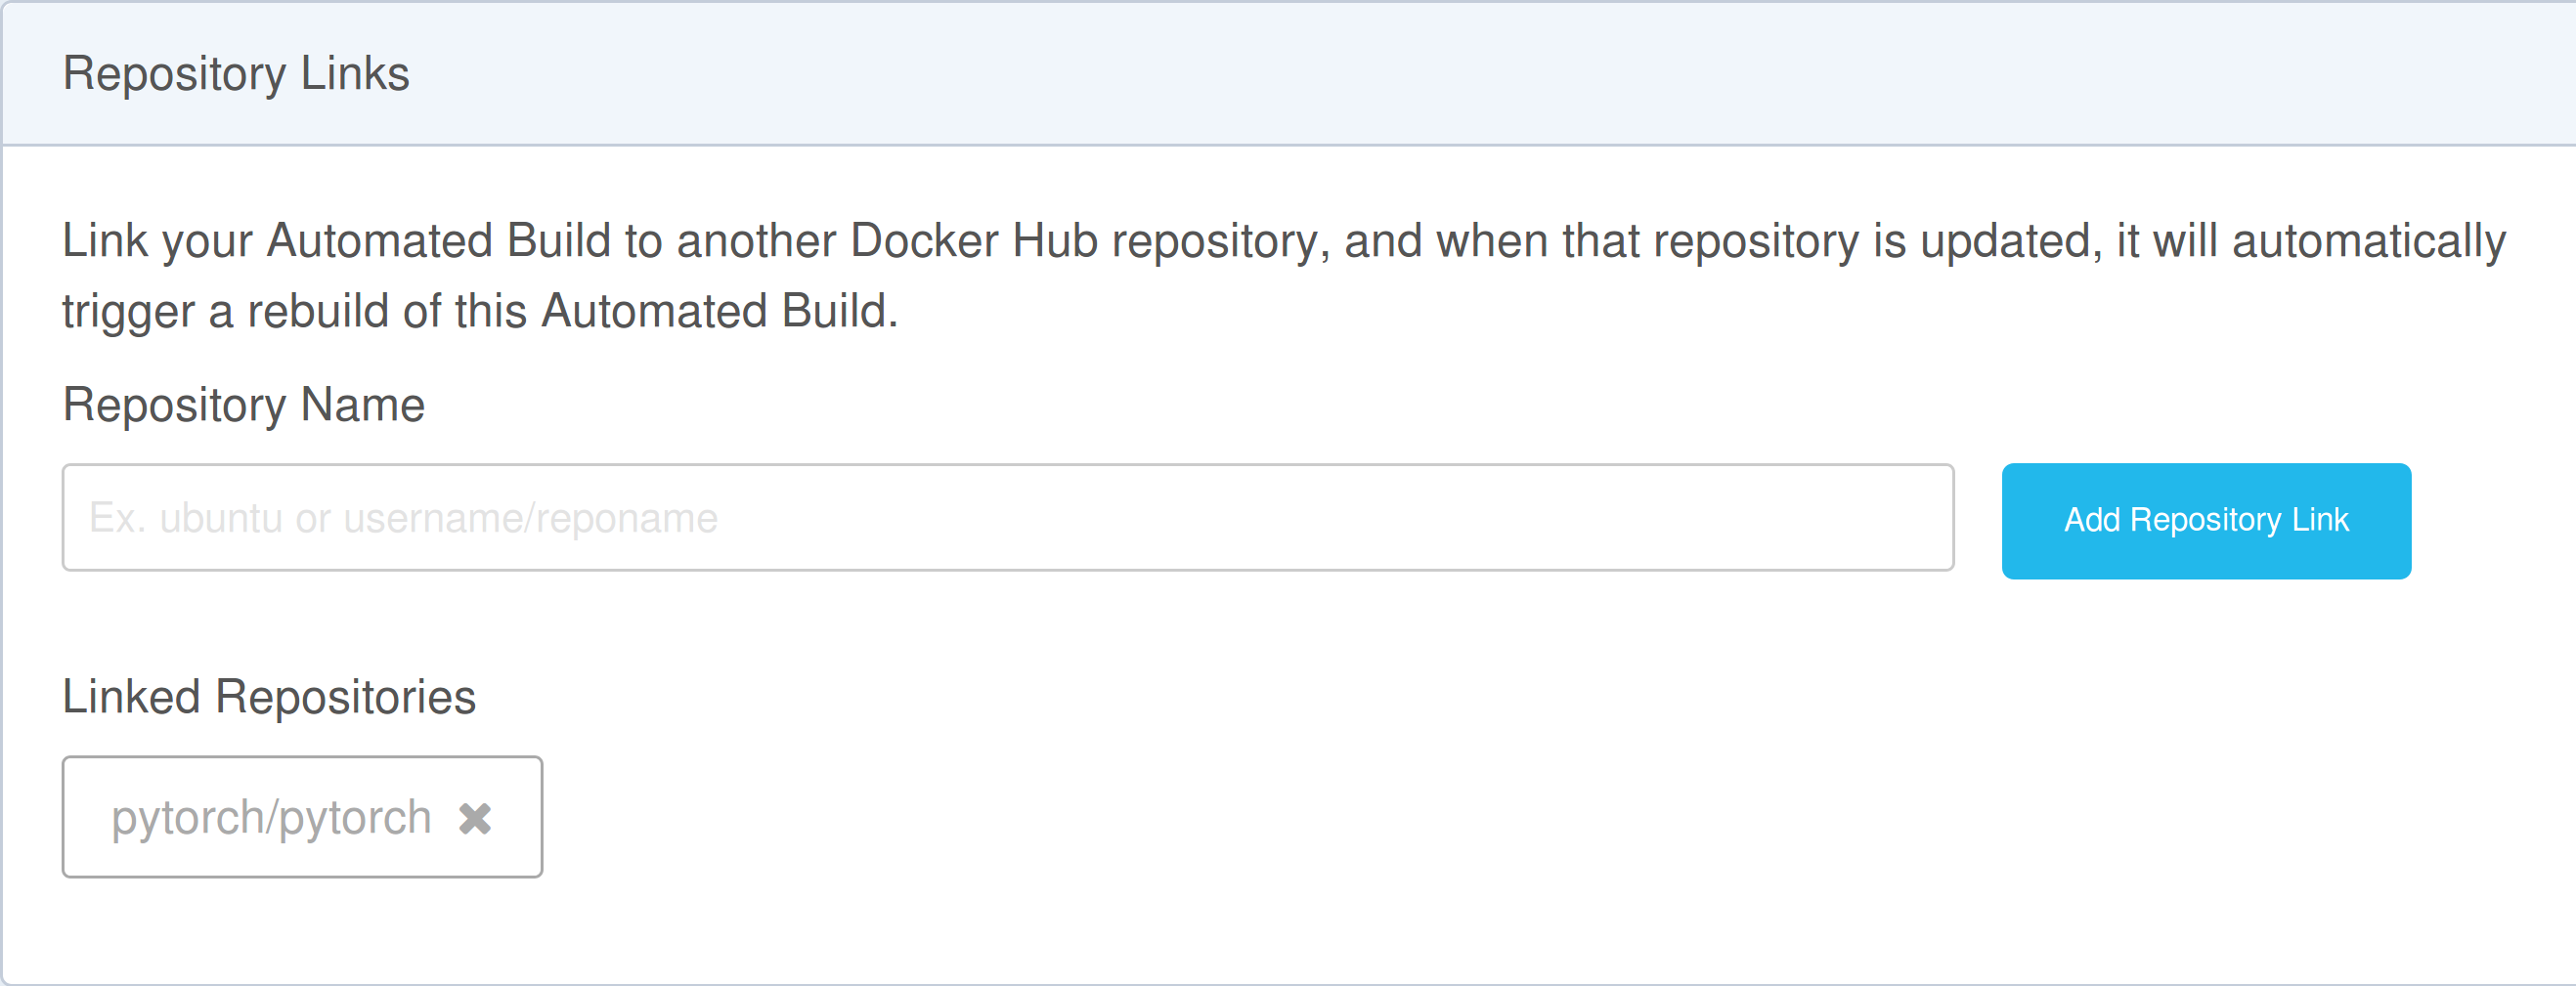
\includegraphics[width=\textwidth]{../figures/docker_hub_repo_links.png}
\end{centering}
%
Repository links allow support chaining builds together across Docker Hub repositories. Whenever a linked repository is updated, the dependent image will be rebuilt.

\subsection{\href{https://cloud.docker.com/}{Docker Cloud}}

Docker Cloud is a Docker registry which is fully integrated with the Docker Hub. Builds are automatically published from Docker Cloud to Docker Hub. Notifications for email and Slack, as well as longer build timeouts (up to 4-hours) are supported. Docker Cloud also supports more advanced build options than Docker Hub, such as a configurable build context and cache settings.\\

\begin{centering}
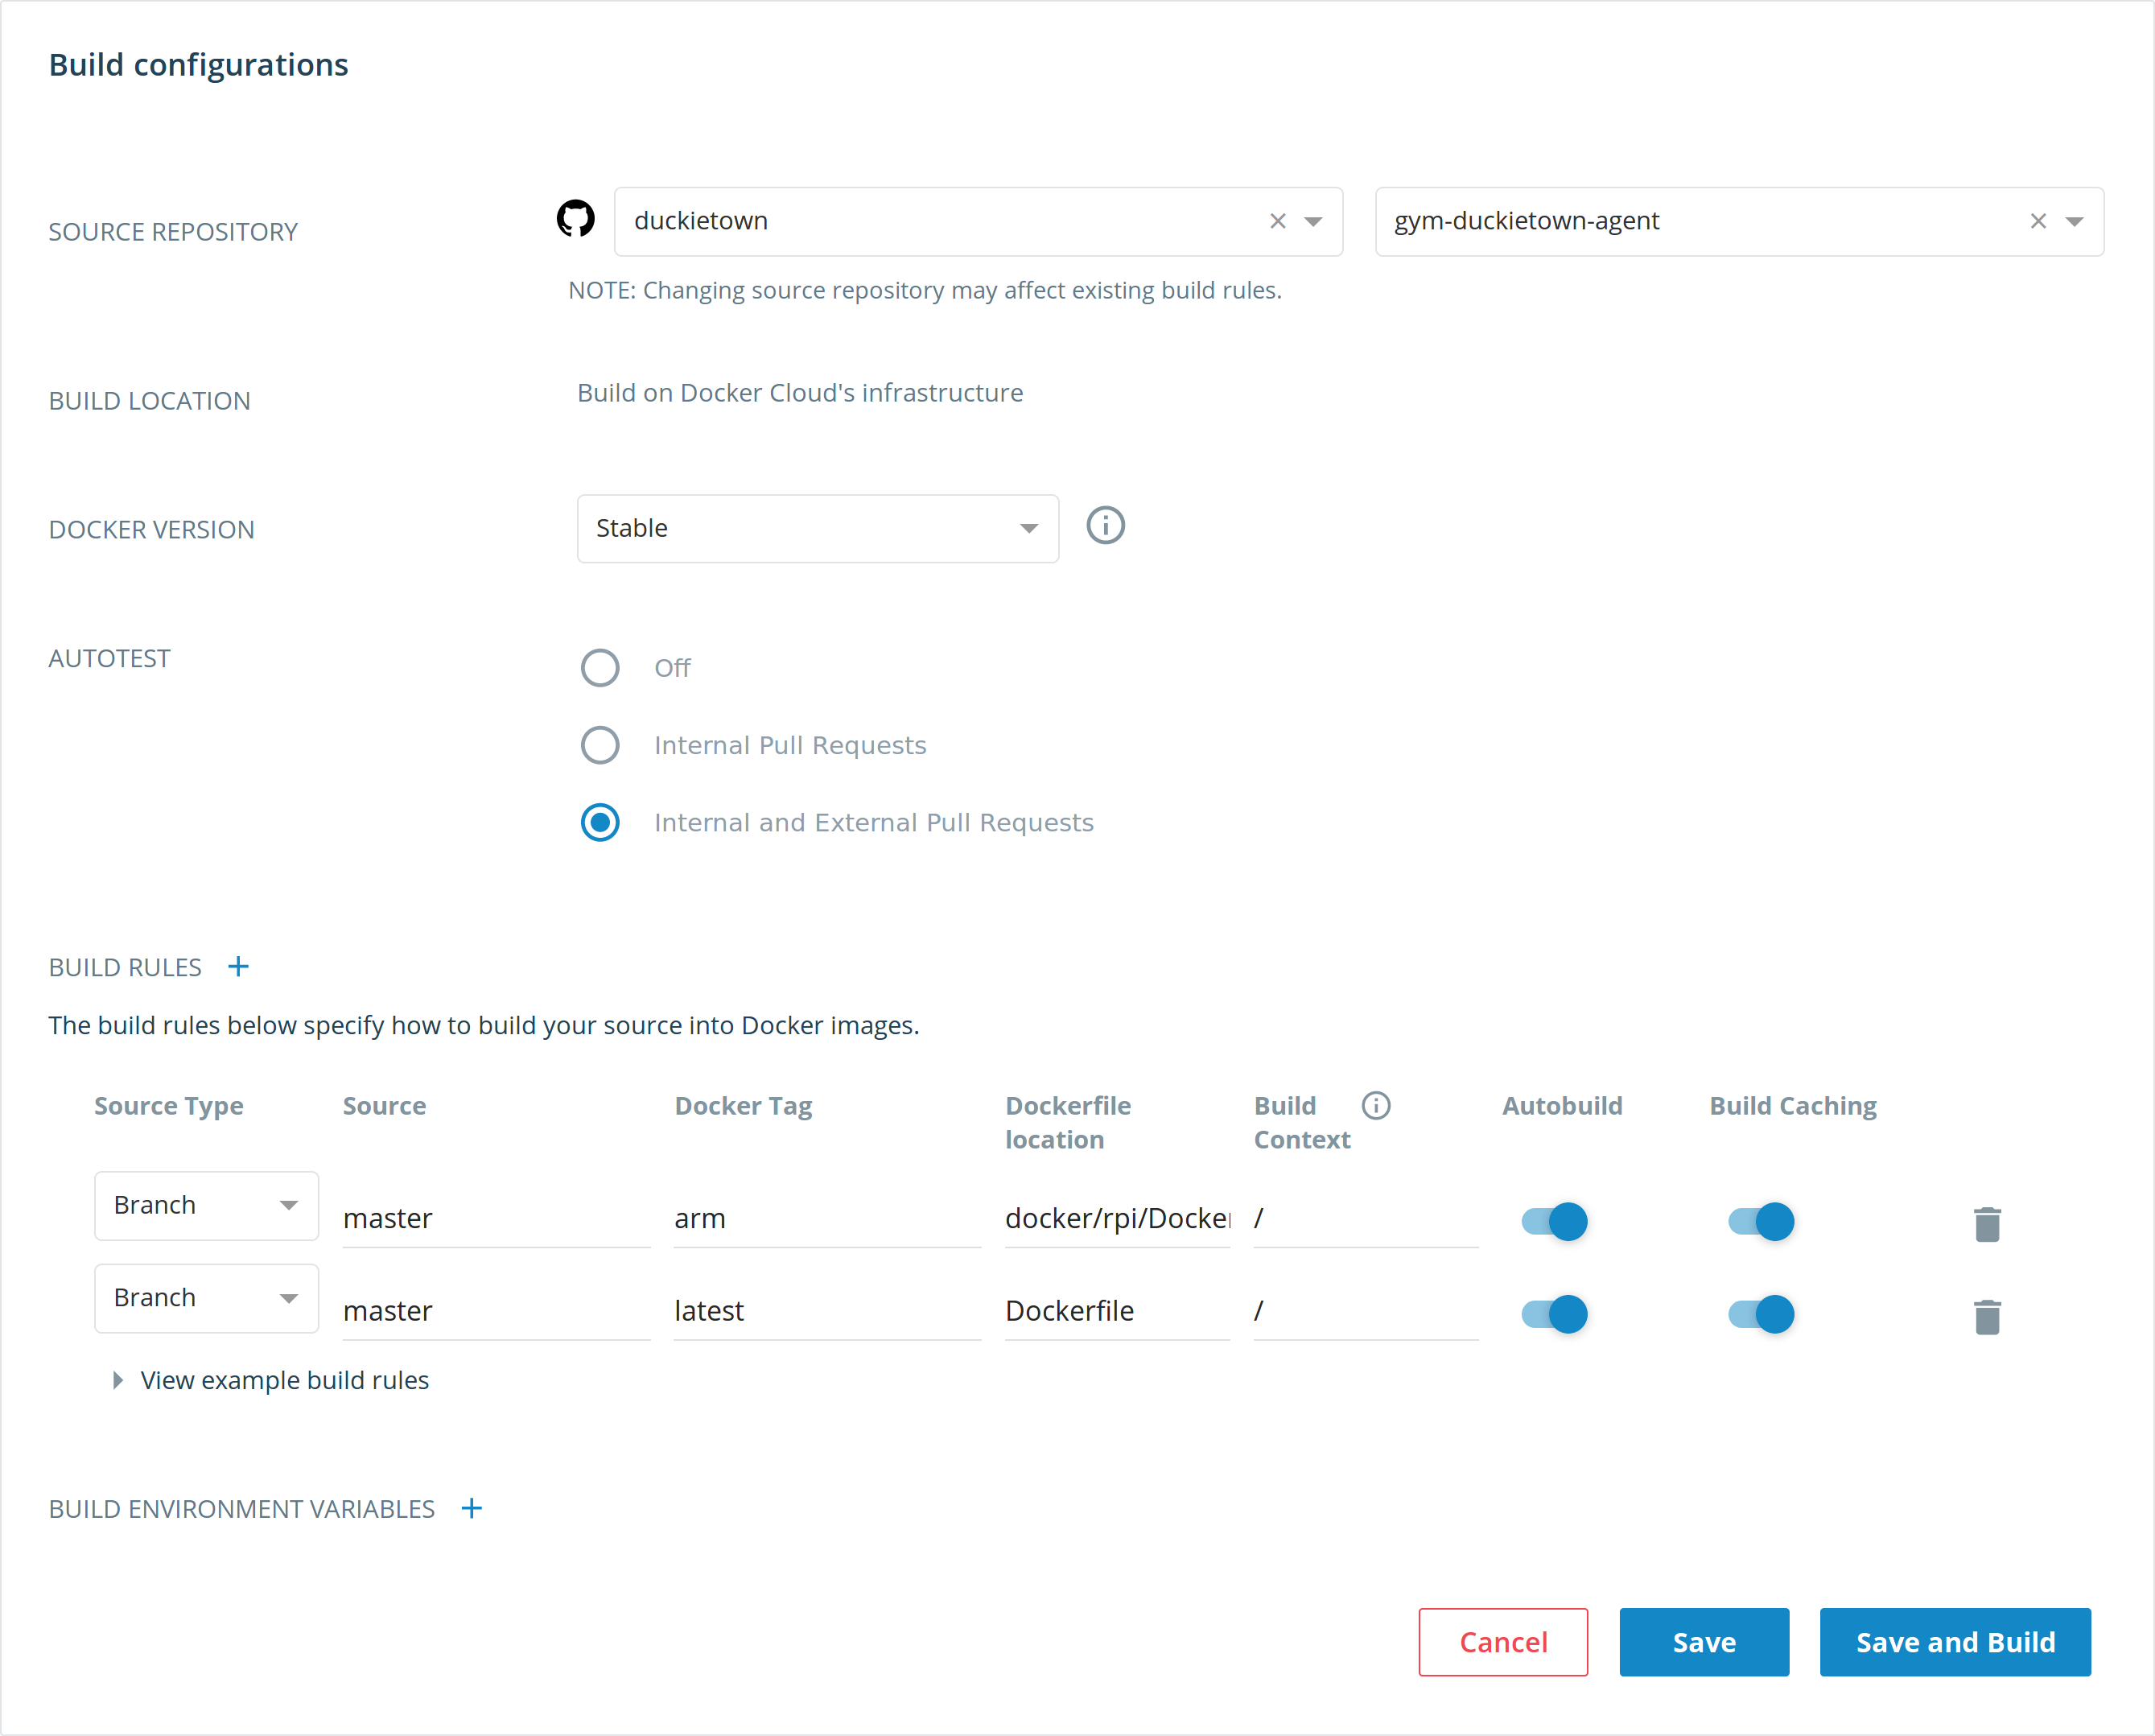
\includegraphics[width=\textwidth]{../figures/docker_cloud.png}
\end{centering}
